\section{Results}
\label{sec:results}

\subsection{Tuning Learning Rate and Minibatch Size}

\subsubsection*{Logistic Regression}
Figure \ref{fig:TuneLogReg_auc} shows a heatmap of the AUC of the Logistic Regression model used on the classification problem for different minibatch sizes and initial learning rates, where the variables are distributed logarithmically.
\begin{figure}[htbp]
	\centering
	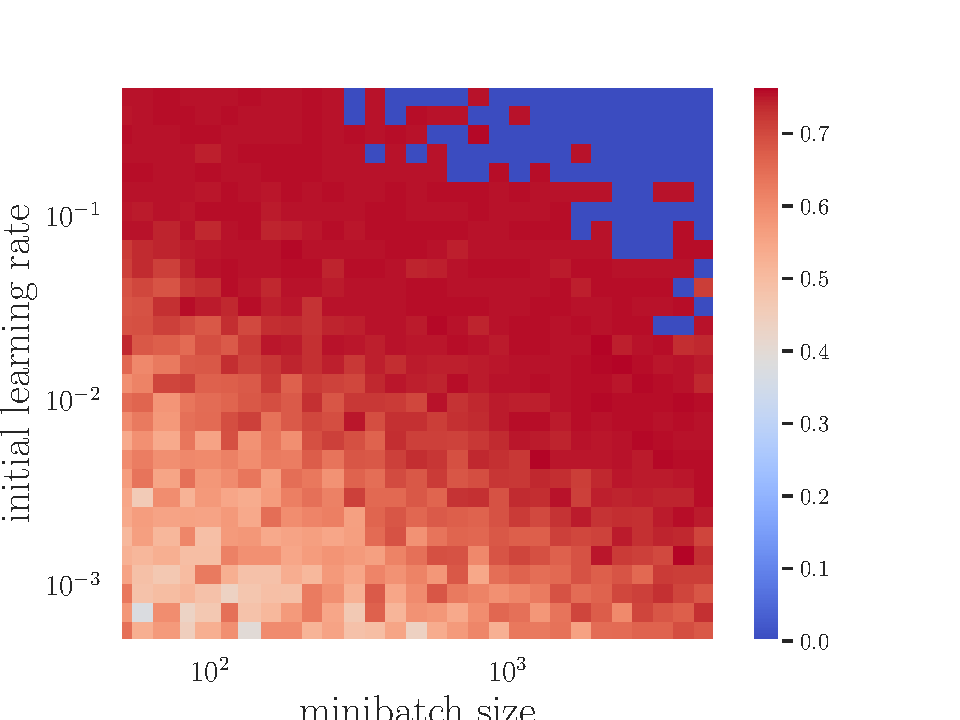
\includegraphics[width=0.5\textwidth]{LogRegTune_auc}
	\caption{Heatmap showing the AUC of the Logistic Regression for different
		values of the minibatch sizes and initial learning rates.}
	\label{fig:TuneLogReg_auc}
\end{figure}

Figure \ref{fig:TuneLogReg_accuracy} is similar to Figure \ref{fig:TuneLogReg_auc}, except that the heatmap shows the accuracy, and not the AUC, for the Logistic Regression.
\begin{figure}[htbp]
	\centering
	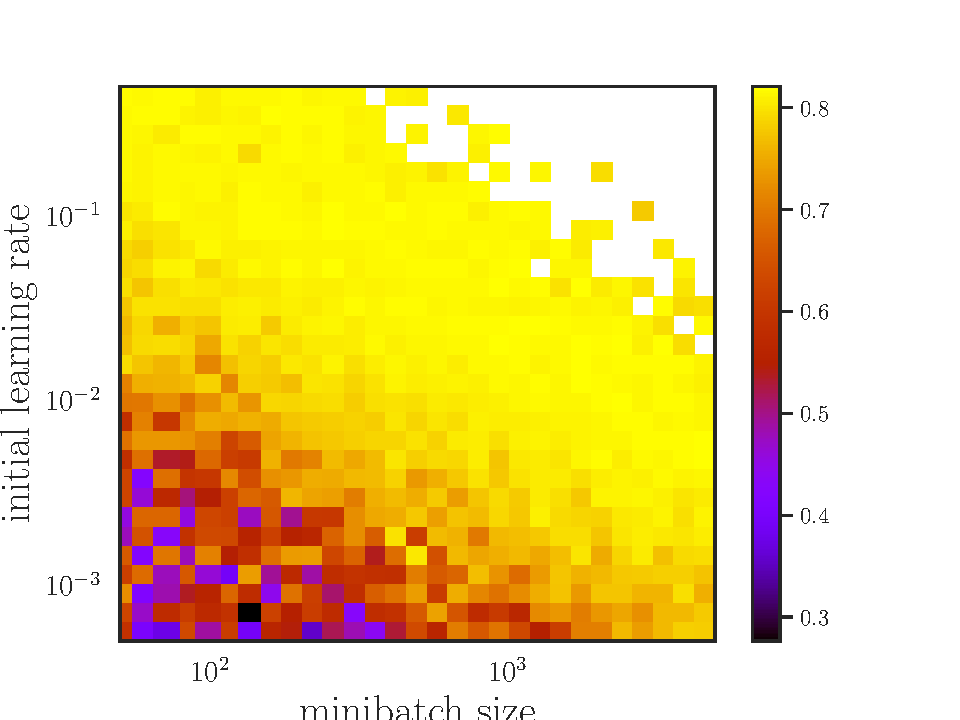
\includegraphics[width=0.5\textwidth]{LogRegTune_accuracy}
	\caption{Heatmap showing the accuracy of the Logistic Regression for different values of the minibatch sizes and initial learning rates.}
	\label{fig:TuneLogReg_accuracy}
\end{figure}

In both Figure \ref{fig:TuneLogReg_accuracy} and \ref{fig:TuneLogReg_auc}, the monochromatic field to the top right represents parameters that gave overflow.

We see that both AUC and accuracy are highest in a band spanning form relatively high initial learning rates and relatively small batch sizes to smaller initial learning rates and larger batch sizes.

\subsubsection*{Neural network}
Figure \ref{fig:TuneNN_accuracy} and \ref{fig:TuneLogReg_auc} shows heatmaps of the accuracy and AUC of the Neural Network.
\begin{figure}[htbp]
	\centering
	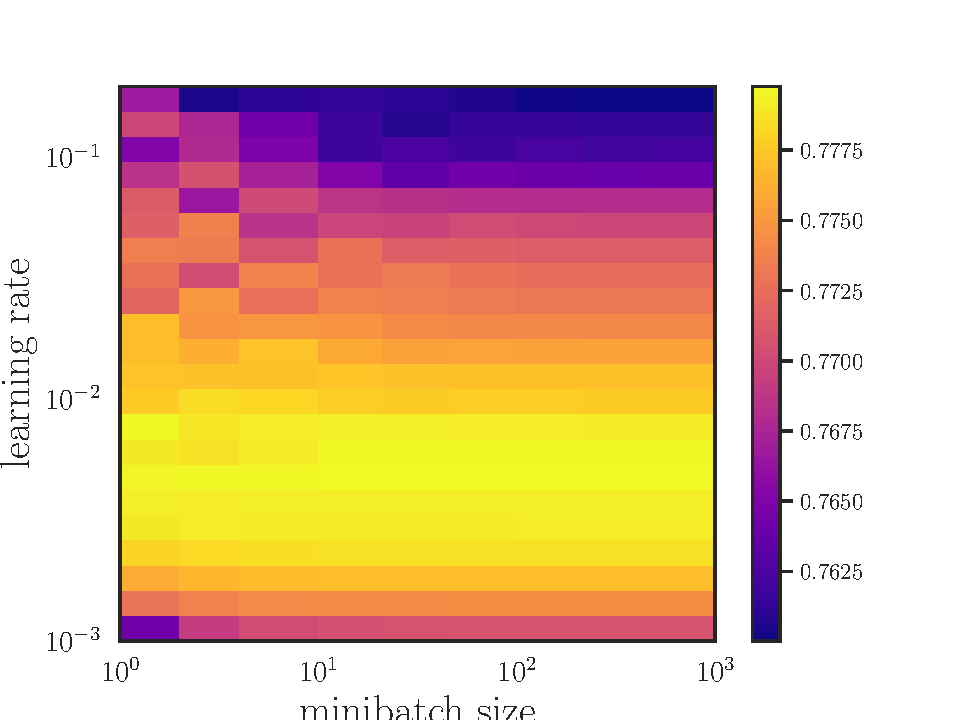
\includegraphics[width=0.5\textwidth]{NNTune_auc}
	\caption{Heatmap showing the AUC of the Neural Network for different
		values of the minibatch sizes and learning rates.}
	\label{fig:TuneNN_auc}
\end{figure}

\begin{figure}[htbp]
	\centering
	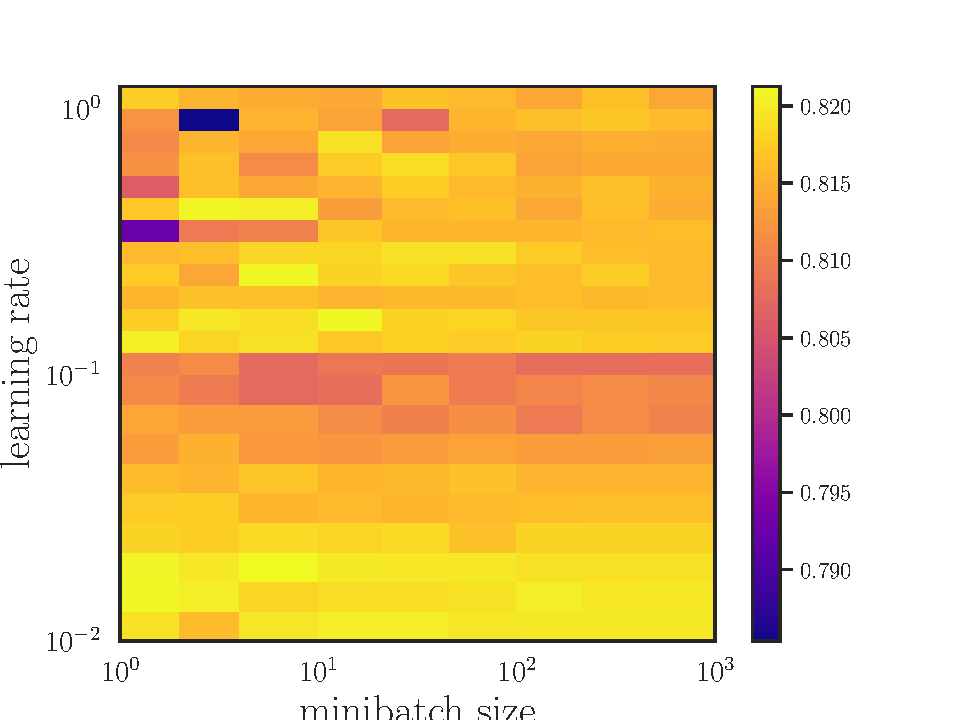
\includegraphics[width=0.5\textwidth]{NNTune_accuracy}
	\caption{Heatmap showing the accuracy of the Neural Network for different
		values of the minibatch sizes and learning rates.}
	\label{fig:TuneNN_accuracy}
\end{figure}

\subsection*{Optimal Parameters and Associated Results}
Table \ref{tab:AUC} spells out the values that gave the highest AUC in Figure \ref{fig:TuneLogReg_auc} and \ref{fig:TuneNN_auc}.
\begin{table}[htbp]
	\renewcommand{\arraystretch}{1.2}
	\caption{Table of parameters that gave the highest \textbf{AUC} in the classification problem. Learning rate $\gamma$, minibatch size m, accuracy acc and AUC is shown for Logistic Regression and Neural Network.}
	\begin{tabular}{p{18mm} p{10mm} p{10mm} p{10mm} p{10mm}}
		\toprule
		Method & $\gamma$ & m & acc & AUC \\
		\midrule
		Logistic \newline regression & 0.15 & 870 & 0.817 & 0.765 \\
		Neural \newline network & 0.035 & 1 & 0.821 & 0.782 \\
		\bottomrule
	\end{tabular}
	\label{tab:AUC}
\end{table}

Similarly, Table \ref{tab:acc} shows the parameters that gave the highest accuracy in Figure \ref{fig:TuneLogReg_accuracy} and \ref{fig:TuneNN_accuracy}.

\begin{table}[htbp]
	\renewcommand{\arraystretch}{1.2}
	\caption{Table of parameters that gave the highest \textbf{accuracy} in the classification problem. Learning rate $\gamma$, minibatch size m, accuracy acc and AUC is shown for Logistic Regression and Neural Network.}
	\begin{tabular}{p{18mm} p{10mm} p{10mm} p{10mm} p{10mm}}
		\toprule
		Method & $\gamma$ & m & acc & AUC \\
		\midrule
		Logistic \newline regression & $0.0069$ & 1645 & 0.820 &  0.758\\
		Neural \newline network & 0.52 & 4 & 0.823 & 0.777 \\
		\bottomrule
	\end{tabular}
	\label{tab:acc}
\end{table}


In Table \ref{tab:confusion}, we can see the number of true and false positives and negatives, when the parameters stated in Table \ref{tab:AUC} are used, i.e. the parameters that gave the highest AUC.
\begin{table}[htbp]
	\renewcommand{\arraystretch}{1.2}
	\caption{Fraction of true and false negatives and positives for Logistic regression, Neural network, and SciKit Learn applied on the classification problem.}
	\begin{tabular}{p{18mm} l l l l}
		\toprule
		Method & \multicolumn{2}{l}{Positive} & \multicolumn{2}{l}{Negative} \\
		\cline{2-3} \cline{4-5}
		& True & False & True & False \\
		\midrule
		Logistic \newline regression & 432 & 210 & 3964 & 776 \\
		Neural \newline network & T466 & 218 & 3956 & 742 \\
		\bottomrule
	\end{tabular}
	\label{tab:confusion}
\end{table}


\subsection{Verification by Comparison to Scikit-Learn}

\subsection{Neural Networks for Regression on Franke's Function}

\begin{figure}[htbp]
	\centering
	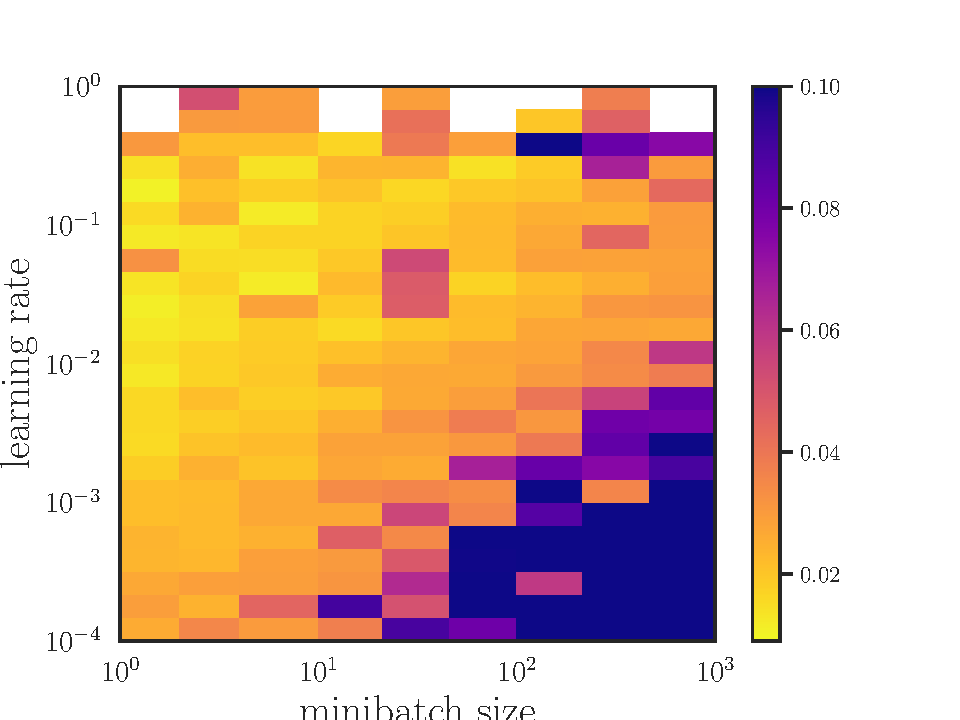
\includegraphics[width=0.5\textwidth]{NNTune_franke_mse}
	\caption{Heatmap showing the MSE of the Neural Network applied on Franke's function for different
		values of the minibatch sizes and learning rates.}
	\label{fig:TuneNN_mse}
\end{figure}
